\section{MODELO ENTIDADE RELACIONAMENTO}

O modelo de dados Entidade-Relacionamento (E-R), visa facilitar o
desenvolvimento do projeto de banco de dados, permitindo a
especificação do esquema de uma base de dados \cite{sistemaDeBancoDeDados}. Na 
Figura \ref{fig:modeloEntidadeRelacionamento}, é apresentado a modelagem do 
banco de dados.

\begin{figure}[h!tb]
	\caption{Modelo Entidade Relacionamento}
	\label{fig:modeloEntidadeRelacionamento}

	\centering
	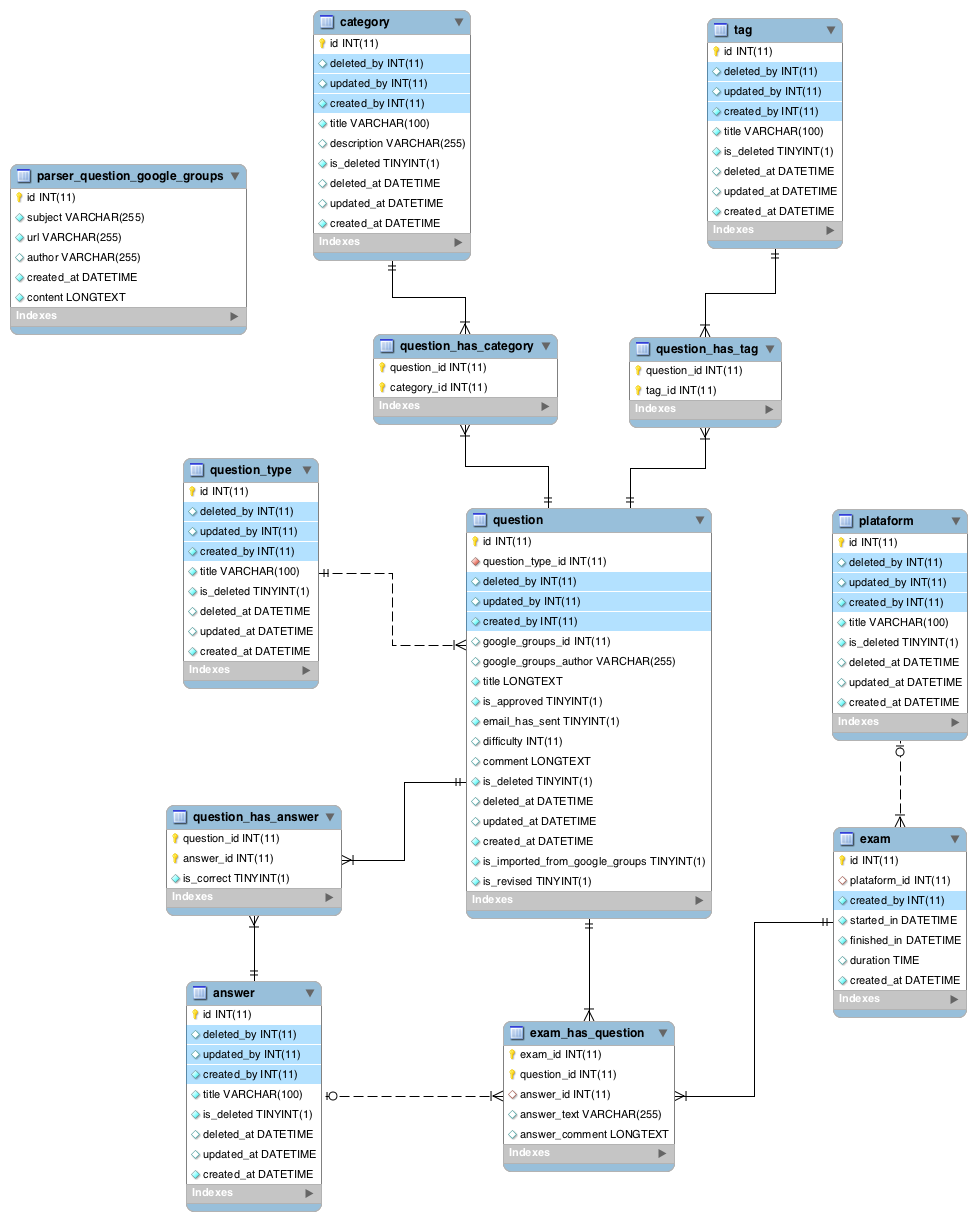
\includegraphics[width=\textwidth]{images/zcpe-reverse-engineer-database.png}

	\centering
	\footnotesize Fonte: \fonteOAutor
\end{figure}

\FloatBarrier 	% Este comando impede que as imagens
				% flutuem a partir deste ponto no seu documento
				
Nota-se que a modelagem do banco de dados apresentada na Figura
\ref{fig:modeloEntidadeRelacionamento} segue um padrão de nomenclatura, e também
evidencia-se que as colunas e tabelas são definidas em inglês, tendo como
objetivo disponibilizar a incentivar a colaboração da ferramenta não apenas a 
nível nacional.
